%!TEX root = ../enrichment.tex
\begin{figure}
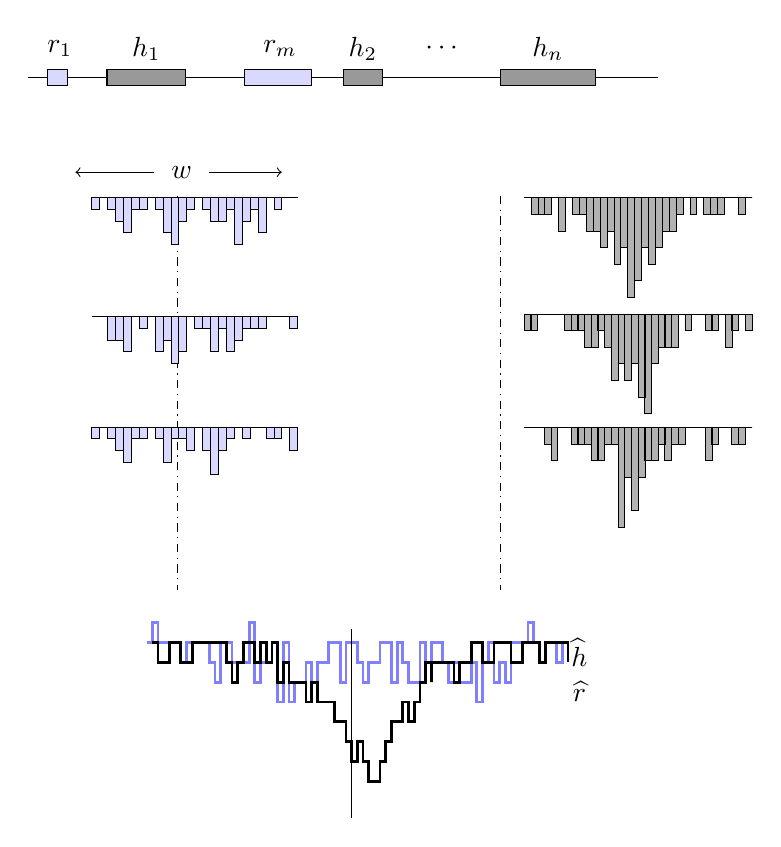
\begin{tikzpicture}
 \draw (0,0) -- (8,0);
 % hotspots
 \draw[fill=black!40] (1,-0.1) -- (2,-0.1) -- (2,0.1) -- (1,0.1) -- cycle;
 \draw[fill=black!40] (4,-0.1) -- (4.5,-0.1) -- (4.5,0.1) -- (4,0.1) -- cycle;
 \draw[fill=black!40] (6,-0.1) -- (7.2,-0.1) -- (7.2,0.1) -- (6,0.1) -- cycle;
 %
 \draw[fill=blue!15] (0.25,-0.1) -- (0.5,-0.1) -- (0.5,0.1) -- (0.25,0.1) -- cycle;
 \draw[fill=blue!15] (2.75,-0.1) -- (3.6,-0.1) -- (3.6,0.1) -- (2.75,0.1) -- cycle;
 % labels
 \node at (1.5,0.37)  {$h_1$};
 \node at (4.25,0.37)  {$h_2$};
 \node at (5.25,0.37)  {$\cdots$};
 \node at (6.6,0.37)  {$h_n$};
 \node at (0.4,0.37) {$r_1$};
 \node at (3.2,0.37) {$r_m$};
%
 \draw[<-] (0.6,-1.2) -- (1.6,-1.2);
 \draw[->] (2.3,-1.2) -- (3.22,-1.2);
 \node at (1.95,-1.2) {$w$};
% vertical lines   
 \draw[dashdotted] (1.9,-1.5) -- (1.9,-6.5);
 \draw[dashdotted] (6,-1.5) -- (6,-6.5);

\begin{axis}[
   at={(0.05\linewidth,-62pt)}, ybar, bar width=2.85pt, width=4.6cm, height=2.3cm,
   axis lines=none
   ]
\addplot[fill=blue!15, line width=0.35pt]%
 coordinates {
  (-2,-1) (-1,0) (0,-1) (1,-2) (2,-3) (3,-1) (4,-1) (5,0) (6,-1) (7,-3) (8,-4) (9,-2) (10,-1) (11,0) (12,-1) (13,-2) (14,-2) (15,-1) (16,-4) (17,-2) (18,-1) (19,-3) (20,0) (21,-1) (22,0) (23,0)
  };
\end{axis}
%
\begin{axis}[
   at={(0.05\linewidth,-145pt)}, ybar, bar width=2.85pt, width=4.6cm, height=2.3cm,
   axis lines=none
   ]
\addplot[fill=blue!15,  line width=0.35pt]%
 coordinates {
   (-2,-1) (-1,0) (0,-1) (1,-2) (2,-3) (3,-1) (4,-1) (5,0) (6,-1) (7,-3) (8,-1) (9,-1) (10,-2) (11,0) (12,-2) (13,-4) (14,-2) (15,-1) (16,0) (17,-1) (18,0) (19,0) (20,-1) (21,-1) (22,0) (23,-2)
 };
\end{axis}
%
\begin{axis}[
   at={(0.05\linewidth,-105pt)}, ybar, bar width=2.85pt, width=4.6cm, height=2.3cm,
   axis lines=none
   ]
\addplot[fill=blue!15,  line width=0.35pt]%
 coordinates {
   (-2,0) (-1,0) (0,-2) (1,-2) (2,-3) (3,-0) (4,-1) (5,0) (6,-3) (7,-2) (8,-4) (9,-3) (10,0) (11,-1) (12,-1) (13,-3) (14,-1) (15,-3) (16,-2) (17,-1) (18,-1) (19,-1) (20,0) (21,0) (22,0) (23,-1)
 };
\end{axis}
%   
%  
%
\begin{axis}[
   at={(0.5\linewidth,-83pt)}, ybar, bar width=2.5pt, width=4.95cm, height=3.1cm,
   axis lines=none
   ]
\addplot[fill=black!30, line width=0.35pt]%
 coordinates {
  (-1,0) (0,-1) (1,-1) (2,-1) (3,-0) (4,-2) (5,0) (6,-1) (7,-1) (8,-2) (9,-2) (10,-3) (11,-2) (12,-4) (13,-3) (14,-6) (15,-5) (16,-3) (17,-4) (18,-3) (19,-2) (20,-2) (21,-1) (22,0) (23,-1) (24, 0) (25,-1) (26,-1) (27,-1) (28,0) (29,0) (30,-1) (31,0)
  };
\end{axis}
%
\begin{axis}[
   at={(0.5\linewidth,-125pt)}, ybar, bar width=2.5pt, width=4.95cm, height=3.1cm,
   axis lines=none
   ]
\addplot[fill=black!30,  line width=0.35pt]%
 coordinates {
  (-1,-1) (0,-1) (1,0) (2,0) (3,-0) (4,-0) (5,-1) (6,-1) (7,-1) (8,-2) (9,-2) (10,-1) (11,-2) (12,-4) (13,-3) (14,-4) (15,-3) (16,-5) (17,-6) (18,-3) (19,-2) (20,-2) (21,-2) (22,0) (23,-1) (24, 0) (25,0) (26,-1) (27,-1) (28,0) (29,-2) (30,-1) (31,0) (32,-1)
 };
\end{axis}
%
\begin{axis}[
   at={(0.5\linewidth,-166pt)}, ybar, bar width=2.5pt,width=4.95cm, height=3.1cm,
   axis lines=none
   ]
\addplot[fill=black!30,  line width=0.35pt]%
 coordinates {
  (-2,0) (-1,0) (0,0) (1,-1) (2,-2) (3,-0) (4,-0) (5,-1) (6,-1) (7,-1) (8,-2) (9,-2) (10,-1) (11,-1) (12,-6) (13,-3) (14,-5) (15,-3) (16,-2) (17,-2) (18,-1) (19,-2) (20,-1) (21,-1) (22,0) (23, 0)  (24, 0) (25,-2) (26,-1) (27,0) (28,0) (29,-1) (30,-1) (31,0)
 };
\end{axis}
% The ``sum'' of all histograms
\begin{axis}[
   width=8cm, height=4cm,
   at={(0.08\linewidth,-260pt)},
   hide x axis,
   hide y axis,
   mark size = 0pt
   ]
\addplot+[const plot, draw=blue!50, line width=1pt]%
 coordinates {
  (-10,0) (-9,1) (-8,-0) (-7,-0) (-6,0)  
  (-5,0) (-4,-1) (-3,-0) (-2,-0) (-1,0)  (0,0)
  (1,-1) (2,-2) (3,-0) (4,-0) (5,-1) 
  (6,-1) (7,-1) (8,1) (9,-2) (10,-1) 
  (11,-1) (12,-0) (13,-3) (14,0) (15,-3) 
  (16,-2) (17,-2) (18,-1) (19,-2) (20,-1) 
  (21,-1) (22,0) (23, 0) (24,-2) (25,0) 
  (26,0) (27,-1) (28,-2) (29,-1) (30,-1)
  (31,0) (32,0) (33,-2) (34,0) (35,-1)
  (36,-2) (37,-2) (38,0) (39,-1) (40,-1)
  (40,-0) (41,-0) (42,-1) (43,-2) (44,-1) 
  (45,-2) (46,-2) (47,-1) (48,-3) (49,-1) 
  (50,0) (51,-2) (52,-1) (53,-2) (54,0)
  (55,0) (56,0) (57,1) (58,0) (59,-1)
  (60,0) (61,0) (62,-1) (63,0) (64,-1)

 };
\addplot+[const plot, draw=black, line width=1pt]%
 coordinates {
   (-9,0) (-8,-1) (-7,-1) (-6,0) (-5,0) 
  (-4,-1) (-3,-1) (-2,-0) (-1,-0) (0,0) 
  (1,0) (2,0) (3,0) (4,-1) (5,-2) 
  (6,-1) (7,0) (8,0) (9,-1) (10,0) 
  (11,-1) (12,-0) (13,-2) (14,-1) (15,-2) 
  (16,-2) (17,-2) (18,-3) (19,-2) (20,-3) 
  (21,-3) (22,-3) (23, -4) (24,-4) (25,-5) 
  (26,-6) (27,-5) (28,-6) (29,-7) (30,-7)
  (31,-6) (32,-5) (33,-4) (34,-4) (35,-3)
  (36,-4) (37,-3) (38,-2) (39,-1) (40,-2)
  (40,-1) (41,-1) (42,-1) (43,-1) (44,-2) 
  (45,-1) (46,-1) (47,0) (48,0) (49,-1) 
  (50,-1) (51,0) (52,0) (53,0) (54,-1) 
   (55,-1) (56,0) (57,0) (58,0) (59,-1)
  (60,0) (61,0) (62,0) (63,0) (64,-1)
 };
\end{axis}
\node at (7, -7.3) {$\widehat h$};
\node at (7,-7.8) {$\widehat r$};
\draw[] (4.11,-7) -- (4.11,-9.4);

\end{tikzpicture}
\label{fig:methodscheme}
\caption{The method}
\end{figure}
